%
% T�TULO DEL CAP�TULO
%
\chapter[ToView]{
	ToView
	\label{chapter_6}
}

ToView is how we named the visualizer that uses PCM under the hood, it was also implemented using C{}\verb!++!, OpenGL for visualization purposes and QT \cite{QT} for the user interface. All of these choices will be explained in the rest of the chapter.

\section[Design]{Design}

The visualizer has been implemented using \textbf{OpenGL 4.3} and \textbf{QT 5.3}. These two technologies were chosen so that the compatibility with multiple platforms was kept. Either OpenGL or QT are compatible with Windows, Linux and MacOS X.

On one hand, OpenGL is an API that allows an application to access and control the graphical system of the machine in which it is being executed. It could be a workstation with a high performance graphics card or a common desktop computer, a video-games console, etc.  

On the other hand, QT is a multi-platform graphical application creation framework. QT is open-source software that has been used and improved since it was created. It fits perfectly with our project since is C{}\verb!++! based. 

QT is used in more than 70 industries, by leading companies in their markets. QT is intuitive, has a suite for the design of interfaces called \textit{QT Designer} and plugins for the major development IDEs like Visual Studio.   

The compilers used as mentioned before are: Visual C{}\verb!++! in Windows systems, GCC in Linux and Clang in MacOS X.

\subsection[GUI]{Graphical User Interface}

\begin{figure}[h]
	\centering
	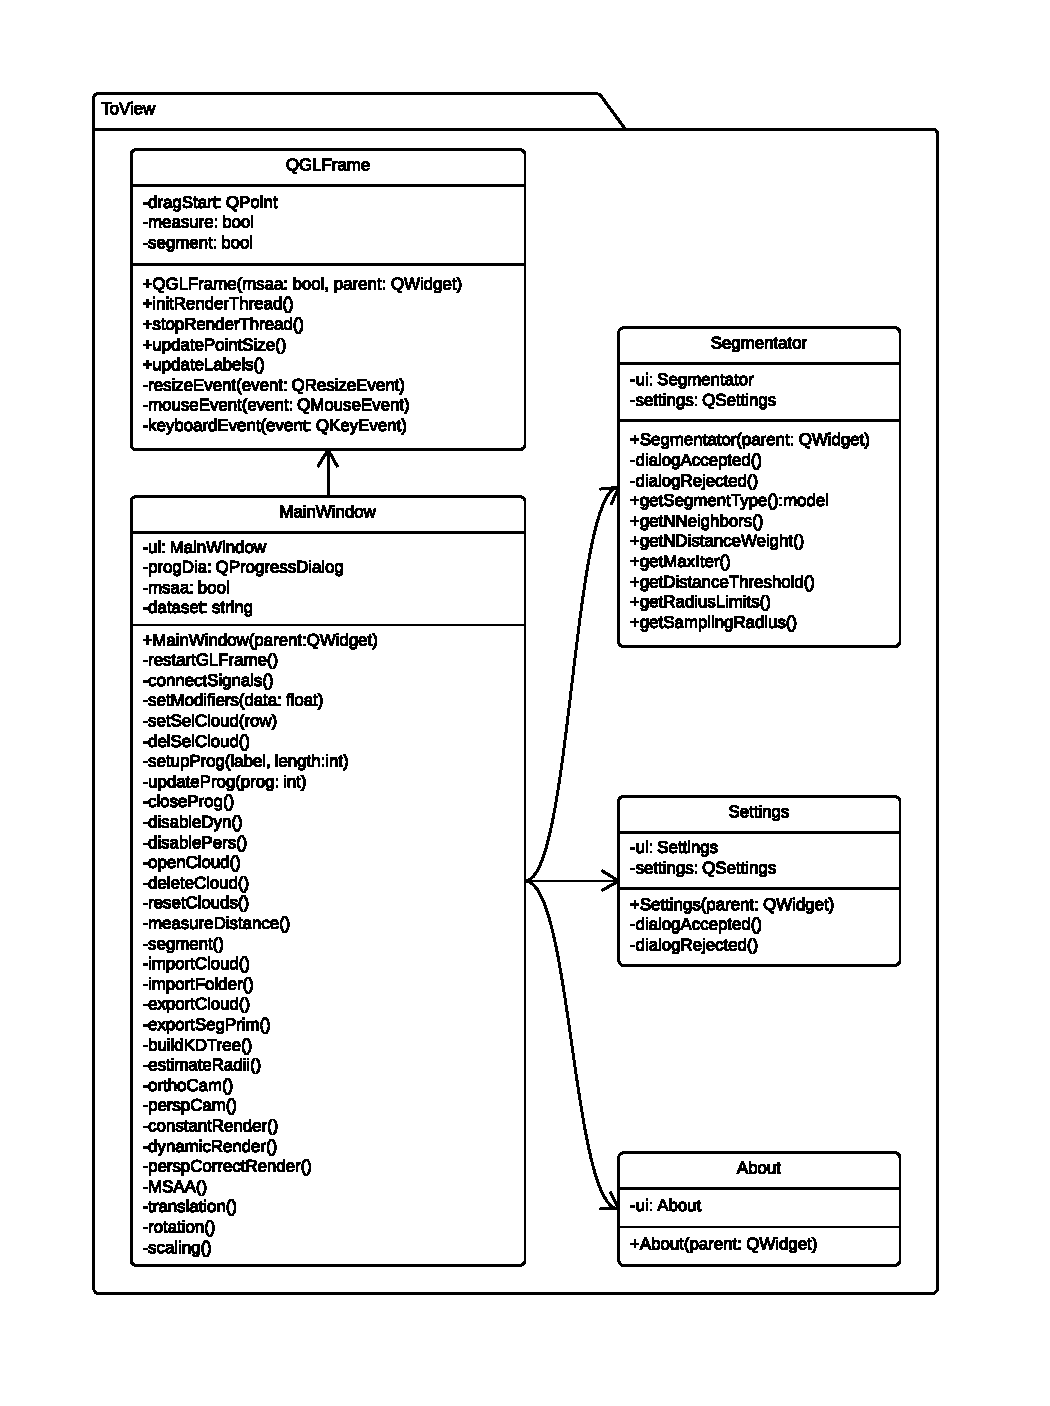
\includegraphics[scale=0.6]{figures/GUI.pdf}
	\caption[User interface class diagram]{
		Class diagram of the user interface of ToView.
	}
	\label{GUI}
\end{figure}

In the \autoref{GUI}, one of the main classes is \textbf{MainWindow}. This class gives the user access to all the functionality of the visualizer, it will serve as the name implies, as the main window in the interface. This class will centralize all the functionality and access to secondary dialogs, as well as communicate with the OpenGL context and render thread. 

The OpenGL context is represented in the interface by the class \textbf{QGLFrame}, that is in charge of creating the corresponding OpenGL context, render thread and displaying each frame rendered. This class will also handle all the keyboard and mouse events.  

The \textbf{Segmentator} class, is a sub-dialog that will let the user input the parameters for the segmentation of primitives in the clouds. All of the choices are saved using the \textbf{Qsettings} class. This QT class simplifies the process of managing settings in an application, eliminating the need for custom configuration files. 

Furthermore, \textbf{Settings} is another sub-dialog that allows the user to configure several visualizer parameters. This dialog also relies on \textbf{QSettings} to store the settings permanently. 

Finally, \textbf{About} is just another sub-dialog that shows information about the software (version, authors, etc.). 

\subsection[Render thread]{Render thread}

\begin{figure}[h]
	\centering
	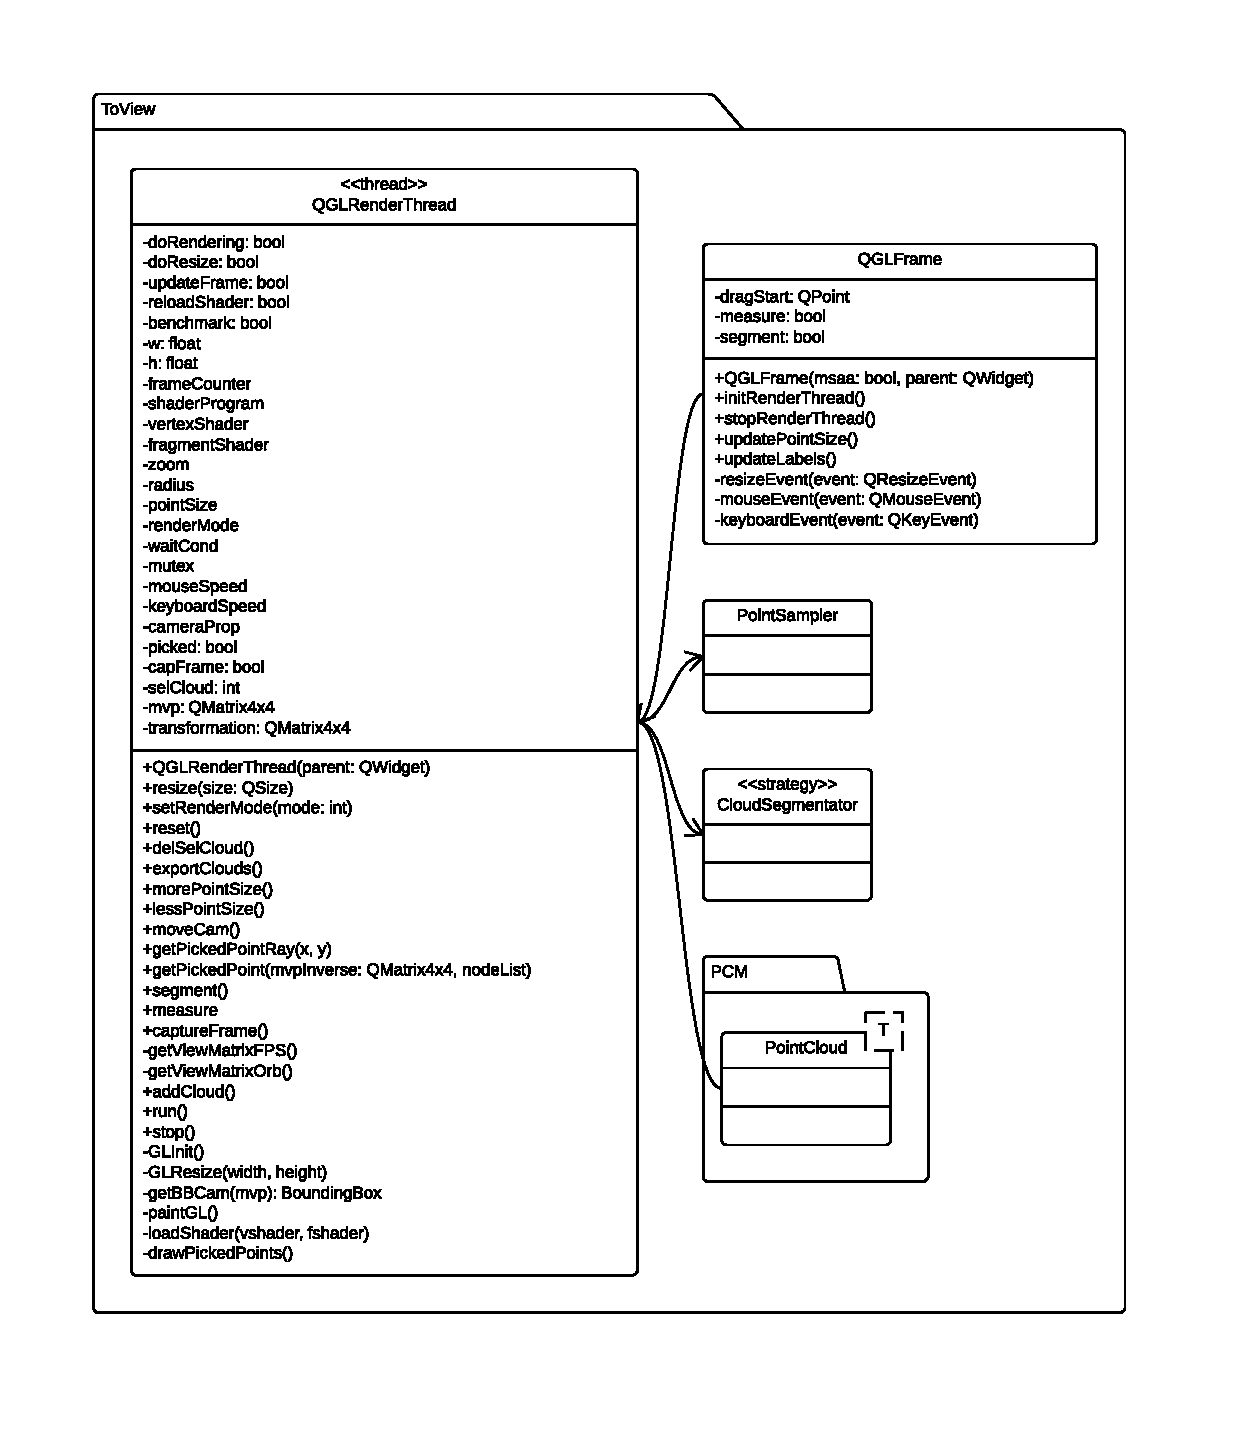
\includegraphics[scale=0.6]{figures/render_thread.pdf}
	\caption[Render thread class diagram]{
		Class diagram of the render thread and its related classes.
	}
	\label{render_thread}
\end{figure}

As we can observe in \autoref{render_thread}, \textbf{QGLRenderThread} is a extremely complex class, that as its name hints, represents a render thread. This class will be in charge of initializing OpenGL, loading shaders, rendering, calculating the camera parameters, etc.

The thread is created by \textbf{QGLFrame}, next the OpenGL context will be transferred to that thread so that the rendering can begin. Rendering is done in a different thread than the GUI, so that the latter will still be responsive even in the most demanding cases. 

Because of this, the communication between the render thread and the GUI will make use of QT \textit{signals} and \textit{slots}\footnote{Language tool introduced in QT for communication between objects, which allows the implementation of the Observer pattern. The concept is that GUI widgets can send signals containing event information, which can be received by other objects using special functions known as slots.}. With these tools, the communication between the different threads will be robust and simpler. Since the render thread could also be used from multiple threads, we will also use a \textit{mutex} to secure concurrent accesses.

To access the cloud information in PCM, the external interface \textbf{PointCloud} is used. \textbf{PointCloud} will provide the necessary information to render the desired clouds; like node lists, point data, memory hierarchy management, etc.      

\subsection[Segmentation]{Segmentation}

\begin{figure}[h]
	\centering
	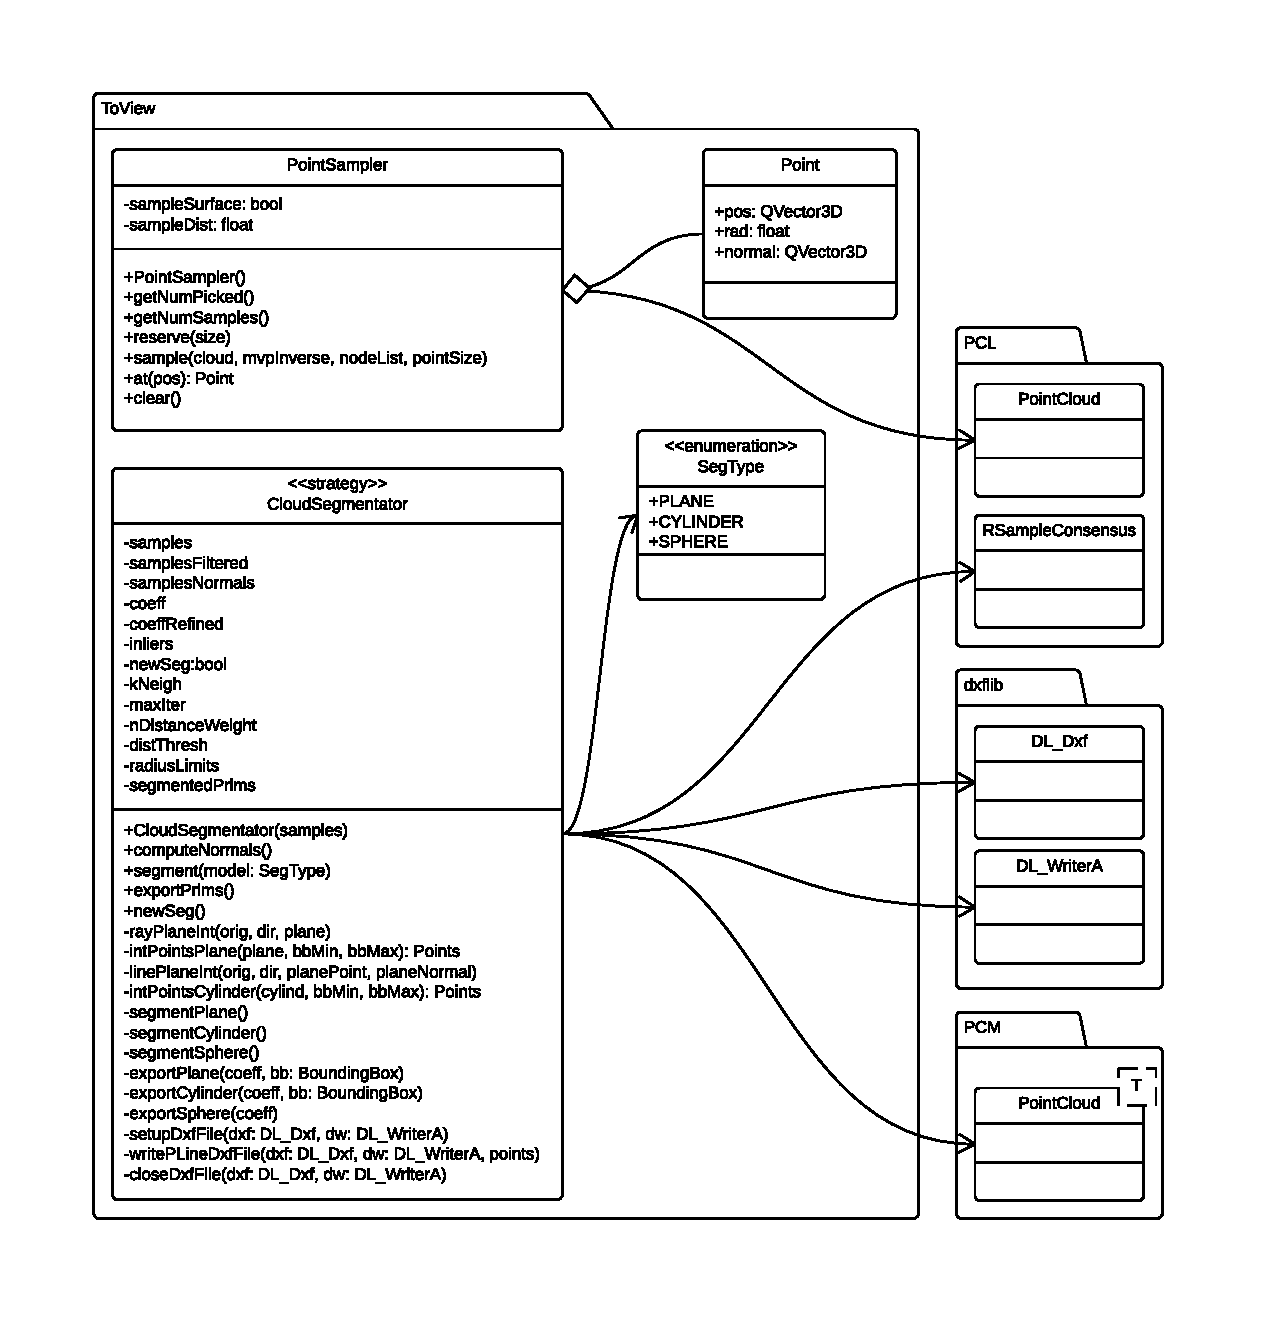
\includegraphics[scale=0.6]{figures/segmentation.pdf}
	\caption[Segmentation class diagram]{
		Class diagram of the classes related to segmentation.
	}
	\label{segmentation_class}
\end{figure}

In \autoref{segmentation_class}, the classes related to the segmentation process are detailed. One of the most significant classes is \textbf{PointSampler}, this will be the class that samples the corresponding point cloud and then converts the data so that it is compatible with PCL. It also is capable of picking individual points for distance measurements, and storing them in a similar fashion to a STL vector for quick access.   

Next, the most important class will be briefly explained. \textbf{CloudSegmentator} uses the information obtained by \textbf{PointSampler} to segment three types of primitives, \textit{planes}, \textit{cylinders} and \textit{spheres}. But this is not all the functionality that this class provides, it is also capable of exporting these primitives to an AutoCAD compatible format. 

To achieve these objectives, this class uses the \textbf{RSampleConsensus} class for primitive fitting and \textbf{DL\_Dxf} for \textit{DXF}\footnote{\textit{Drawing Exchange Format} is a CAD data file format developed by Autodesk for enabling data interoperability between AutoCAD and other programs.} exporting. Since there is not a good way to export cylinders and spheres in the DXF format, the segmentator will also support exporting these primitives as \textit{SCR}\footnote{\textit{Script Files} are simply a list of AutoCAD commands.} files.

Since some of the primitives need normals for the segmentation process, \textbf{CloudSegmentator} also includes the capability to estimate them. The pattern \textit{Strategy} was used for the design of this class so that adding primitives in the future will be easy. 
